\section{Design}
\label{sec:design}

The Multisurf system has three main components:
\begin{itemize}
\item The browser extension which interacts with the user.
\item The native client application which is responsible for communicating with the peers and for performing the integrity checks.
\item The peer application which mirrors any requests from the Multisurf client.
\end{itemize}

The browser extension gathers HTTP request and response data while the user browses the web normally.
In the background, the Multisurf extension passes this information to the native client, which solicits all received HTTP requests via SSL to one or more trusted peers.
These also issue the same request for a web page to the web server.
The peer returns its version of the server’s served content to the client.
Figure \ref{fig:protocol} details the client-peer protocol.

To perform the integrity check, the Multisurf client compares the original server web page content with the peers' versions of the request web page.
We have designed various comparison vectors which the client can employ to verify the integrity of the received content for the request web page:
\begin{itemize}
\item A line-by-line comparison of the content. This is a rather coarse-grained comparison metric.
\item The number of script tags in the content. Any discrepancies in this could indicate a malicious script injection.
\item The links contained within \texttt{<script>} tags and \texttt{<a>} tags. This algorithm finds matching elements in the web content being compared. Differing links in the same element may indicate a malicious in-flight injection.
\end{itemize}

The client sends the result of the consistency check back to the browser extension, which displays the results to the user.
In the case of an unsafe website, the browser extension allows the user to view the differing web pages to help her determine if she deems the differences malicious or not.
Should the user decide that an unsafe website is malicous, the extension allows her to blacklist the site for future browsing sessions.

\begin{figure}[h]
\centering
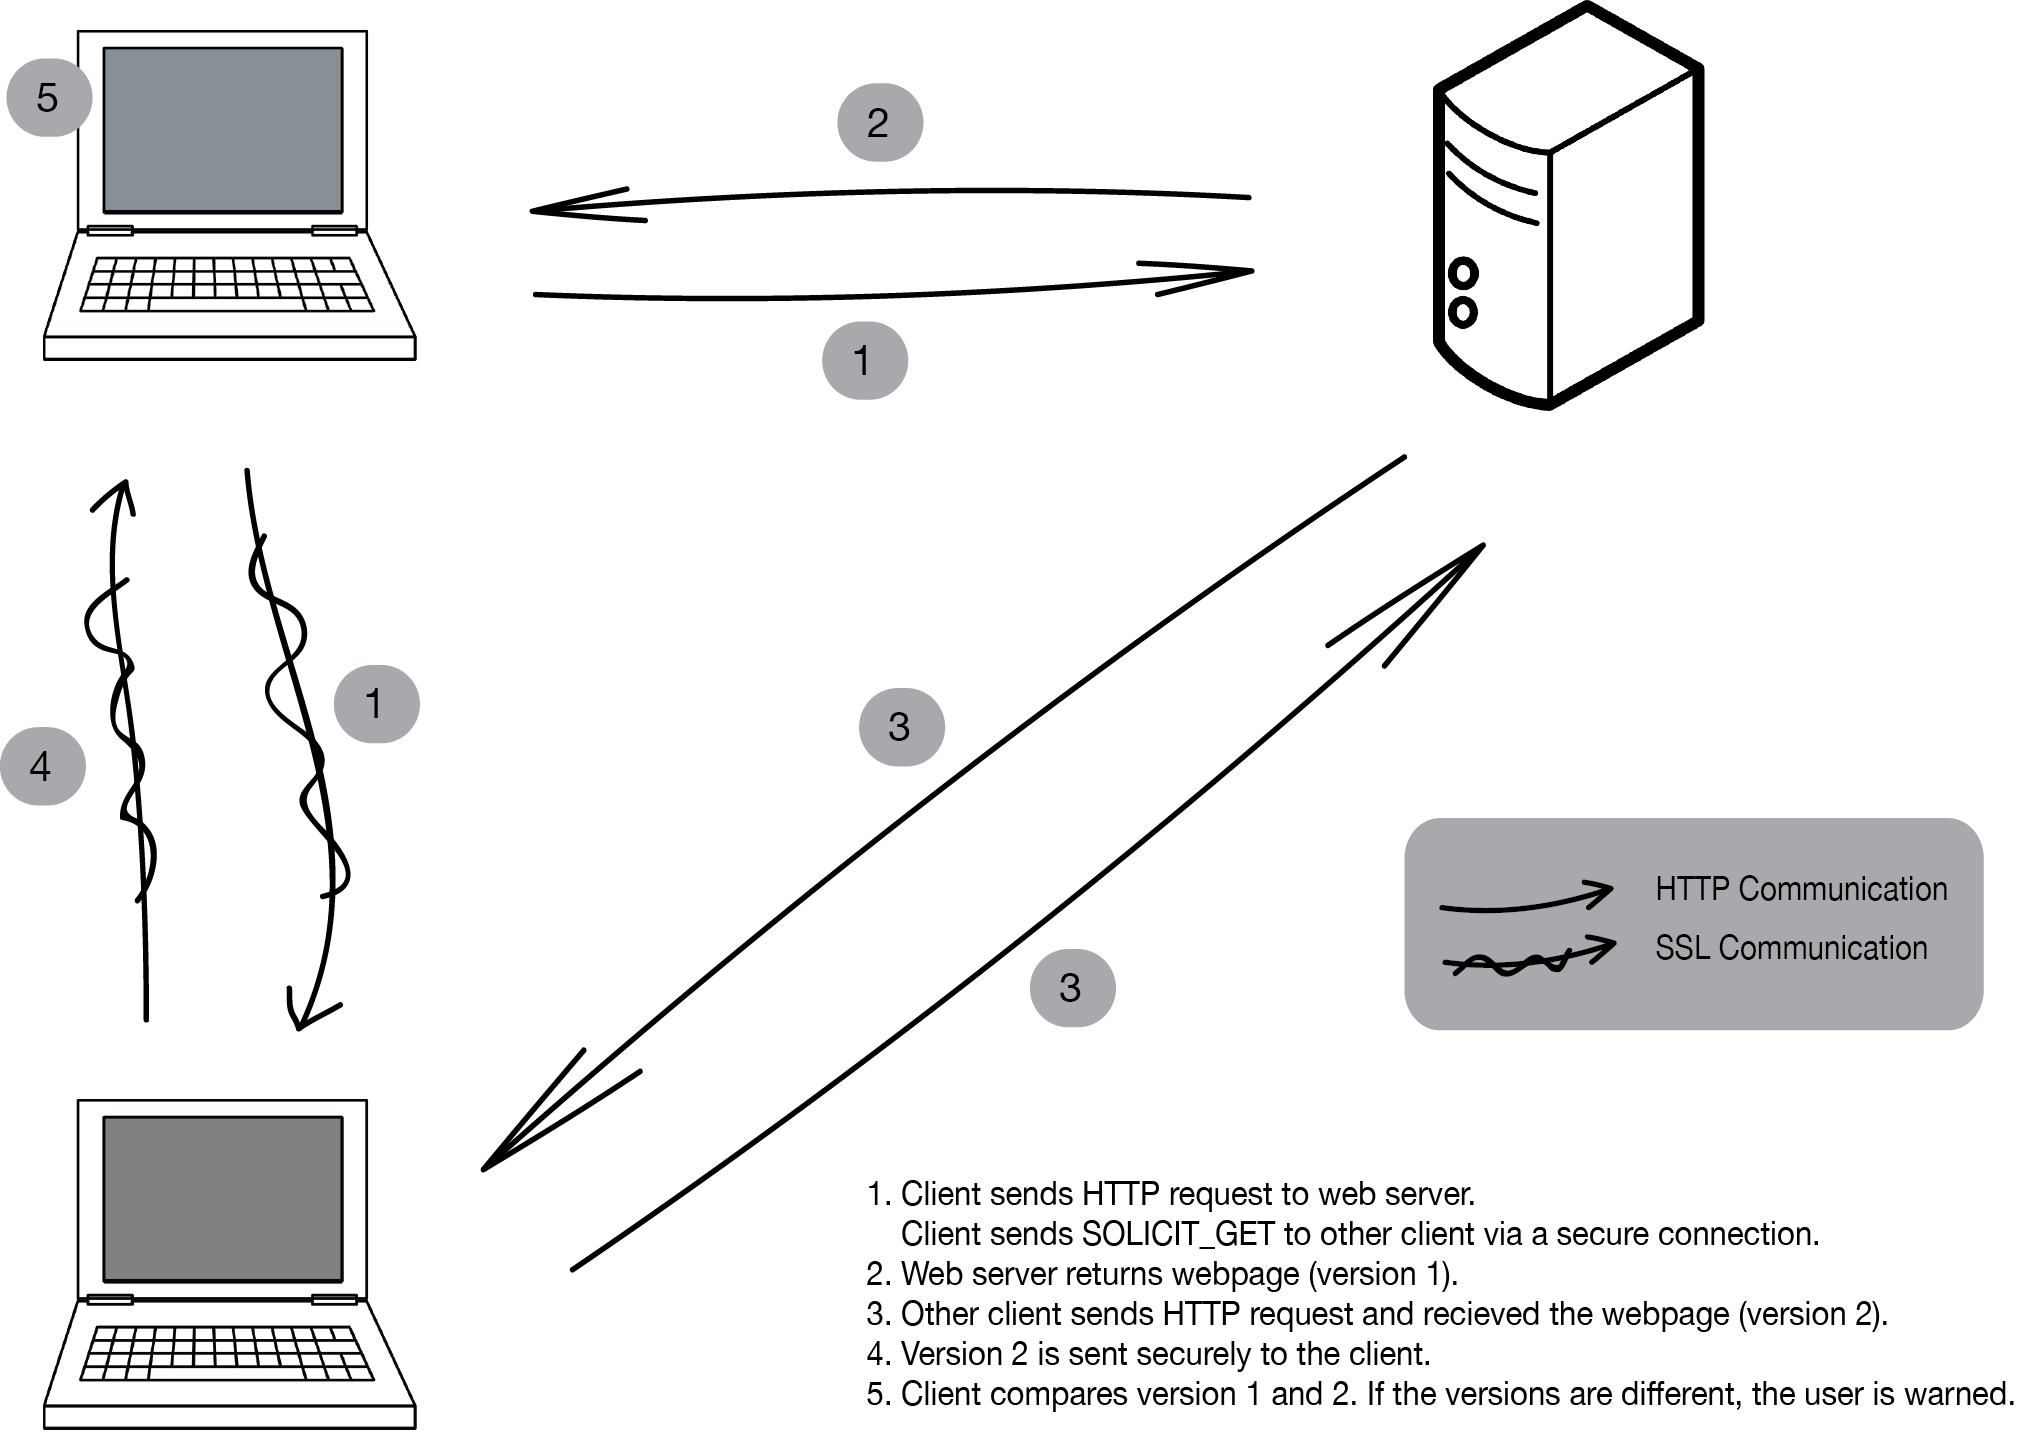
\includegraphics[scale=0.4]{./Protocol.png}
\caption{The Multisurf client-peer protocol.}
\label{fig:protocol}
\end{figure}

\subsection{Implementation}
We have implemented a working Multisurf prototype. The browser extension is implemented for the Google Chrome browser in Javascript and Python. The native client and peer applications are implemented in Python. We have made our code available on Git Hub.\footnote{\url{http://github.com/ohadf/multisurf}}